\subsection{Dados de Validação}
Os dados de validação são os meses após os dados de treino, de Janeiro 2024 ao fim de Agosto 2024.\par
Usamos como \textit{benchmark} as capacidades alocadas, "\textit{SecondaryReserveAllocationAUpward}" e "\textit{SecondaryReserveAllocationADownward}", e como validação e objectivo, \hyperref[se:metneuralnet]{y}, a própria energia usada, "\textit{UpwardUsedSecondaryReserveEnergy}" e "\textit{DownwardUsedSecondaryReserveEnergy}".

\textbf{Benchmark}

Como método de comparação a todas as experiências foi criado uma base que servirá de \textit{benchmark}.\par
Este base não é nada mais do que a própria previsão feita pela entidade reguladora \gls{ESIOS}. Dentro do nossos dados correspondem aos valores nos campos "\textit{SecondaryReserveAllocationAUpward}" e "\textit{SecondaryReserveAllocationADownward}".\par
Para os dados utilizados, podemos ver a totalidade e comparação do \textit{benchmark} (Energia Alocada) com a energia utilizada.\par

\begin{figure}[H]
    \centering
    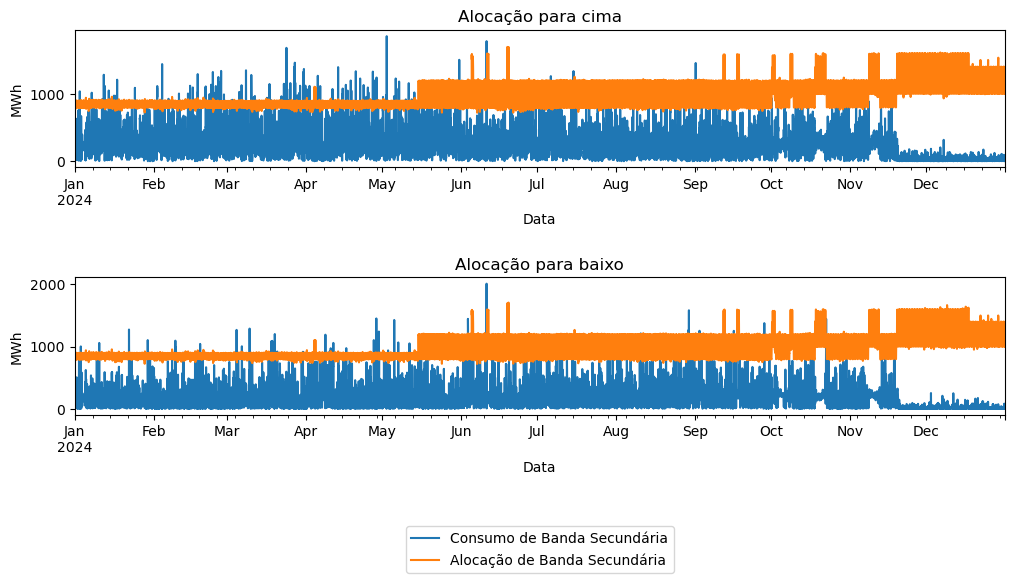
\includegraphics[width=0.6\textwidth]{plots/benchmark_alocacoes_validacao.png}
    \caption{Série Temporal dos dados de Benchmark c/ consumo real}
    \label{fig:benchmarktimeseries}
\end{figure}

Os valores alocados no período de validação mantêm um dinamismo fixo entre dois pontos, seguindo um formula não dinamica. \par
Mas o mais importante a notar é a forma estática destes métodos, que, em virtude da natureza flutuante da energia necessária, apresentam, frequentemente um erro grande.\par
Tal é possível de verificar através da análise de algumas janelas temporais dentro do período de validação, em concreto, atentando no melhor e pior resultado, em termos de erro absoluto, em janelas temporais de ano, mês, semana e dia.\par


\begin{figure}[H]
    \centering
    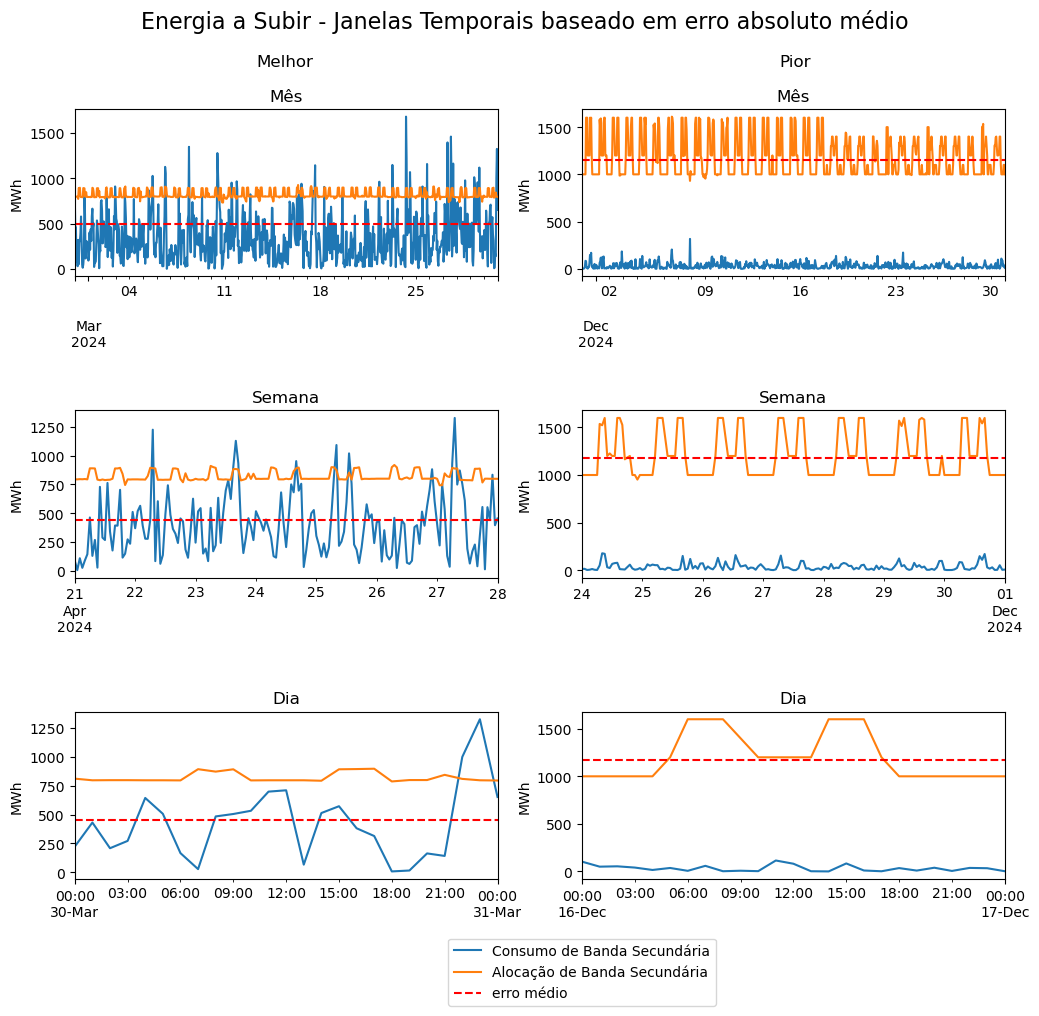
\includegraphics[width=0.7\textwidth]{plots/alocacoes_temporais_upward_dataset.png}
    \caption{Janelas temporais de \textit{benchmark} energia a subir}
    \label{fig:benchmarktimewindowsup}
\end{figure}


\begin{figure}[H]
    \centering
    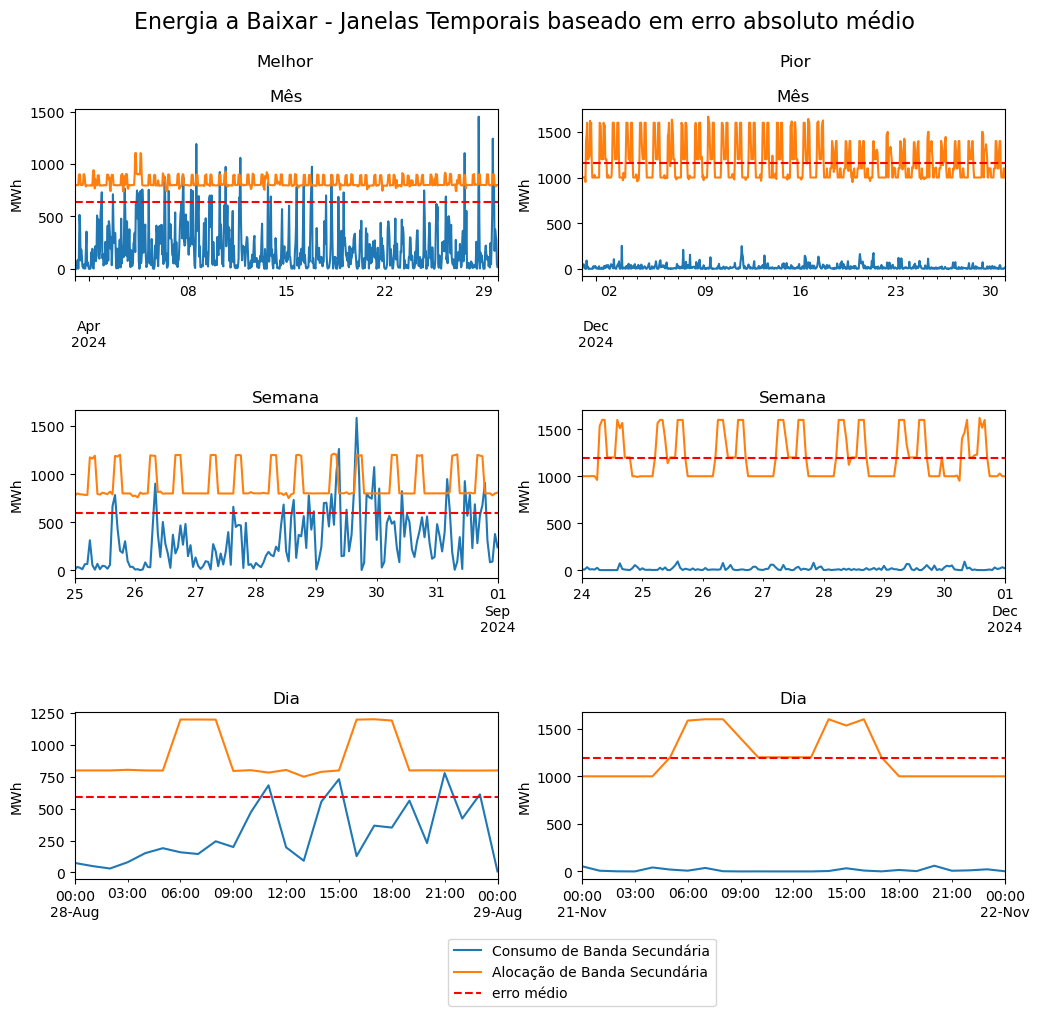
\includegraphics[width=0.7\textwidth]{plots/alocacoes_temporais_downward_dataset.png}
    \caption{Janelas temporais de \textit{benchmark} energia a descer}
    \label{fig:benchmarktimewindowsdown}
\end{figure}

Dentro destas janelas temporais conseguimos ter melhor a percepção da natureza estática deste modelo actual, e quão longe está dos valores reais necessários.\par

Os resultados a melhorar são:\\
\begin{table}[H]
    \centering
    \caption{Resultados métricas \textit{benchmark}}    
    \resizebox{0.8\linewidth}{!}{\begin{table}[H] 
    \caption{This is a table caption. Tables should be placed in the main text near to the first time they are~cited.\label{tab1}}
    \newcolumntype{C}{>{\centering\arraybackslash}X}
    \begin{tabularx}{\textwidth}{CCCCC}
    \toprule
    & \textbf{RMSE}	& \textbf{SAE}	& \textbf{AllocF} & \textbf{AllocD}\\
    \midrule
    Up Allocation (MW) & 536.55 & 17357826.75 & 152679.00 & 17205147.75 \\
    Down Allocation (MW) & 408.99 & 12981575.55 & 479191.60 & 12502383.95 \\
        \bottomrule
    \end{tabularx}
    % \noindent{\footnotesize{\textsuperscript{1} Tables may have a footer.}}
\end{table}

}
    \label{tab:benchmarkmetrics}
    \end{table}

As correlações entre o método actual e a energia consumida podem ser vistas na figura abaixo:\\


\begin{figure}[H]
    \centering
    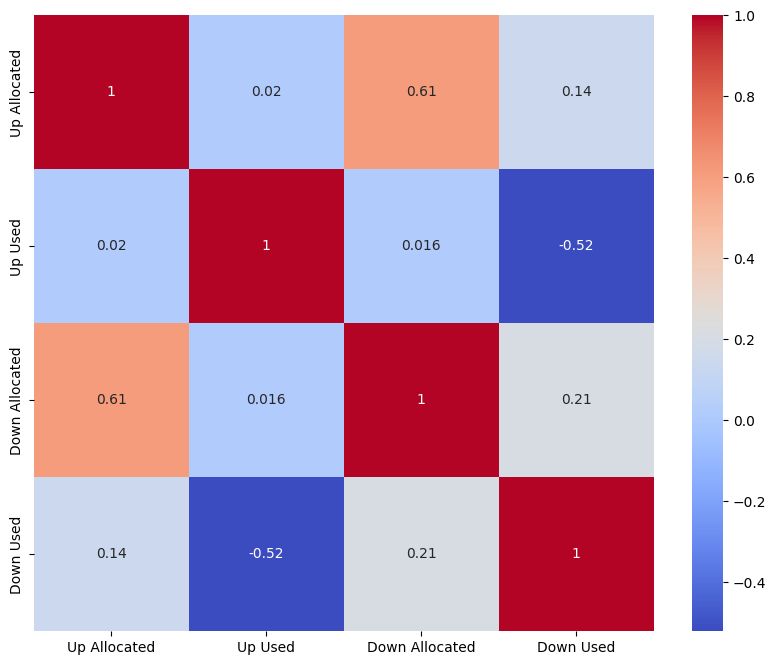
\includegraphics[width=\textwidth]{plots/correlation_heatmap_benchmark.png}
    \caption{Correlação entre \textit{benchmark} e real}
    \label{fig:benchmarkcorr}
\end{figure}

% TODO: meter formula da previsão ENTO-e no capitulo estudo 2 -> nao existe publicamente
Neste período de validação, a energia alocado para cima é igual a alocada para baixo. com uma correlação de 1, diferente da totalidade dos dados disponíveis em que as alocações mostram uma correlação de 58\%.
As relações entre as energias alocadas são altas devido à natureza do \hyperref[]{método de previsão} enquanto que a correlação entre a energia alocada e a usada são bastante baixas com 23\% na alocaçao a descer e 9,8\% na alocação a subir.\par
O que não mostra uma ligaçao entre as alocações e a energia usada, mas apenas entre as energias alocadas.\par

